% CSC 300: Professional Responsibilities
% Dr. Clark Turner

% Two Column Format
\documentclass[11pt]{article}
%this allows us to specify sections to be single or multi column so that things
% like title page and table of contents are single column
\usepackage{multicol}

\usepackage{graphicx}
\usepackage{dblfloatfix}
\usepackage{fixltx2e}

\usepackage{setspace}
\usepackage{url}

%%% PAGE DIMENSIONS
\usepackage{geometry} % to change the page dimensions
\geometry{letterpaper}

\begin{document}

\title{\vfill Maintenance Courses in a Software Engineering Curriculum} %\vfill gives us the black space at the top of the page
\author{
James Pearson \vspace{10pt} \\
CSC 300: Professional Responsibilities  \vspace{10pt} \\
Section 1 \vspace{10pt} \\
Dr. Clark Turner \vspace{10pt} \\
}
%\date{October 22, 2010} %Or use \Today for today's Date
\date{\today}

\maketitle

\vfill  %in combinaion with \newpage this forces the abstract to the bottom of the page
\begin{abstract}
Although software maintenance makes up most of the work a software engineer will do in the workplace, Cal Poly requires Software Engineering undergraduates to take only two courses that cover software maintenance.  Considering this, is it ethical for the Computer Science department to state that the program is designed to produce software professionals?  The ACM's Software Engineering Code of Ethics lists maintenance as one of the primary focuses for a Software Engineer; given this, the department should require a more thorough instruction in the art of software maintenance for Software Engineering students.
\end{abstract}

\thispagestyle{empty} %remove page number from title page
\newpage


%Create a table of contents with all headings of level 3 and above.
%http://en.wikibooks.org/wiki/LaTeX/Document_Structure#Table_of_contents has
%info on customizing the table of contents
\thispagestyle{empty}  %Remove page number from TOC
\tableofcontents

\newpage

%end the 1 column format


%start 2 column format
\begin{multicols}{2}
%Start numbering first page of content as page 1
\setcounter{page}{1}
%%%%%%%%%%%%%%%%%%%%
%%% Known Facts  %%%
%%%%%%%%%%%%%%%%%%%%
\section{Facts}

The Cal Poly catalog states that the Software Engineering undergraduate degree ``prepares students to become software professionals who develop software 
products on time, within budget, and that meet customer requirements''. \cite{catalogDept}  It also says that the program differs from the similar Computer Science undergraduate degree program in four ways, one of which is having ``classes [that] include significant learning in engineering and management areas such as quality assurance, testing, metrics, maintenance, configuration management and interpersonal management skills.'' \cite{catalogDept}

CSC 309's course description refers to ``maintenance of large software systems'', while CSC 406's simply mentions ``software maintenance''.\footnote[1]{Three courses in the Computer Science department's section of the 2011-13 Cal Poly Catalog have the word ``maintenance'' in their course description. \cite{catalogCourses}  In one of these, CSC 358 Computer System Administration, the reference is to ``system maintenance''. \cite{catalogCourses}  Given the course title and that the course is billed as teaching ``fundamental concepts of Unix system administration'', \cite{catalogCourses} we can conclude that the maintenance described is of an operating system and its components, rather than a single piece of software in which the maintainer is altering code.  Thus, this course is not of relevance to our discussion.} \cite{catalogCourses}

George E. Stark claims that ``maintenance consumes between 60 percent and 80 percent of a typical product's total software lifecycle expenditures''. \cite{stark97}  Girish Parekh says that it is two-thirds of the lifecycle and consumes at least 50 percent of most programmers' time. \cite{parekh}

Andrews and Lutfiyya, while preparing in 1998 for a software maintenance course at the University of Western Ontario, found no courses at other universities in which students performed maintenance activities on legacy software. \cite{andrews} They also found that ``most computer science programs offer[ed] no more than two software engineering course''. \cite{andrews}

%%%%%%%%%%%%%%%%%%%%%%%%%
%%% Research Question %%%
%%%%%%%%%%%%%%%%%%%%%%%%%
\section{Research Question}

Does the Cal Poly Software Engineering program include enough training in software maintenance in CSC 309 and CSC 406?

Cal Poly requires Software Engineering undergraduates to take only two courses whose course descriptions cover software maintenance, and those courses are designed to teach about several other topics as well. \cite{catalogCourses}  However, the ACM Software Engineering code of ethics lists software maintenance as one of the roles of a software engineer \cite{secode}, and studies have shown that software maintenance consumes a large portion of the software life cycle. \cite{stark97} \cite{parekh}

%%%%%%%%%%%%%%%%%%%%%%%%%
%%% Extant Arguments from External Sources %%%
%%%%%%%%%%%%%%%%%%%%%%%%%
\section{Extant Arguments}

\subsection{Arguments For}

Andrews and Lutfiyya found that their software maintenance course ``gave students valuable experience in the qualitatively different task of software maintenance''. \cite{andrews}  Engle, Ford and Korson state that it is ``important for students to have experienced [software maintenance]''. \cite{engle}

\subsection{Arguments Against}

\subsubsection{Difficulty of Classroom Instruction}

Engle, Ford and Korson's project stemmed from a perceived ``difficulty of preparing a software system upon which maintenance can be performed''; their end product consisted of 10,000 lines of Ada code and 9 documents. \cite{engle}

Andrews and Lutfiyya avoided creating a large maintenance-ready system by involving several clients and working on free software projects under the GNU Project.  One student team had both their first and second projects cancelled due to a lack of available time on the part of the client; this meant they had to switch to new projects twice during the term. \cite{andrews}

In addition, Andrews and Lutfiyya faced complications in grading; each group was working on a different project and each had its own goals. \cite{andrews}  Grades could not even be fairly assigned based on the clients' satisfaction, as one group unknowingly implemented a feature that had been previously finished (but without an updated status in the project wiki). \cite{andrews}

Andrews and Lutfiyya also noted issues with finding available projects that would be stable enough that student code would not be irrelevant by the end of the course, yet new enough to be using cutting-edge technologies that the students were enthusiastic about. \cite{andrews}

% Talk about issues with iRobot in 2011 Capstone?

\subsubsection{Cost of Increasing Maintenance Coverage in Existing Courses}

One of the Cal Poly courses that covers software maintenance, CPE 309, also covers several other topics:

\begin{quote}
Methods and tools for the implementation, integration, testing and maintenance of large software systems. Software development and test environments. Software quality assurance. \cite{catalogCourses}
\end{quote}

CPE 406, the other course, similarly covers a range of topics:

\begin{quote}
Deployment of a sizeable software product by a student team. Software maintenance and deployment economic issues. Management of deployed software: version control, defect tracking and technical support. \cite{catalogCourses}
\end{quote}

According to our current understanding of mathematics, increasing the coverage of one subject while holding the total time constant necessitates that time must be taken away from the other subjects.  That is, adjusting the breakdown of a currently-offered course without adding more units will always be a tradeoff - an increase in one subject corresponds to a decrease in another.  If the department does not wish to decrease time spent on any other subjects, they cannot increase the time spent on software maintenance without adding another course.

\subsubsection{Cost of a New Course}

The Cal State University system has faced continuous budget cuts over the last decade, reaching its lowest level of funding since 1998. \cite{tuitonFall}  Correspondingly, yearly fees for an in-state student rose from \$2976 in 2002 to over \$7900 for students entering in Fall 2011 \cite{feeHistory} and there has been an almost 9\% decrease in the number of CSU employees since 2008. \cite{tuitonFall}

Cal Poly students have had difficulty in registering for their classes as it is. \cite{scramble}  Adding an additional course requires the department to either replace a section of another course (making that other course more difficult to enroll in) or find the resources for another room and professor.

Cal Poly has not released any statistics about the cost of a course; we do know, however, the salaries of professors.  For instance, Dr. Turner received a salary of \$99,672.00 in 2011. \cite{sacbee}  From scheduling information, he appears to teach 5 4-unit courses a year. \cite{TurnerSchedule}  This places an estimate of roughly \$20,000 for a course he teaches.  In addition, the school must arrange access to a room, provide it with electricity, and perform any necessary maintenance and cleaning.

%%%%%%%%%%%%%%%%
%%% Analysis %%%
%%%%%%%%%%%%%%%%
\section{Analysis}

\subsection{Applicability of the SE Code}

This paper will use the ACM's Software Engineering Code of Ethics as a basis for evaluating the ethicality of the Computer Science department's course offerings.  Therefore, we must first show that the SE Code may be applied to the department.

The preamble to the Code explicitly states that it applies to those engaged in the education of software engineers:

\begin{quote}
``Software engineers are those who contribute by direct participation or by teaching, to the analysis, specification, design, development, certification, maintenance and testing of software systems''. \cite{secode}
\end{quote}

A few sentences later, it reaffirms this:

\begin{quote}
``The Code contains eight Principles related to the behavior of and decisions made by professional software engineers, including [...] educators''. \cite{secode}
\end{quote}

% SE Code: ``Software engineers are those who contribute by direct participation or by teaching, to the analysis, specification, design, development, certification, maintenance and testing of software systems.''

``The Computer Science Department educates students in the discipline of computer science'' and has an ``educational mission''. \cite{catalogDept}  Although we will make no claim that computer science is the same as software engineering, the department also claims that ``[t]he BS in Software Engineering prepares students to become software professionals''. \cite{catalogDept}  Therefore, the Computer Science department of Cal Poly falls under the educator category of those the SE Code wishes to regulate.

% 1.06. Be fair and avoid deception in all statements, particularly public ones, concerning software or related documents, methods and tools.
% 2.01. Provide service in their areas of competence, being honest and forthright about any limitations of their experience and education.
% 3.01. Strive for high quality, acceptable cost and a reasonable schedule, ensuring significant tradeoffs are clear to and accepted by the employer and the client, and are available for consideration by the user and the public.
% 3.04. Ensure that they are qualified for any project on which they work or propose to work by an appropriate combination of education and training, and experience.
% 3.11. Ensure adequate documentation, including significant problems discovered and solutions adopted, for any project on which they work.
% 3.15. Treat all forms of software maintenance with the same professionalism as new development.
% 5.06. Attract potential software engineers only by full and accurate description of the conditions of employment.
% 5.11. Not ask a software engineer to do anything inconsistent with this Code. (professors as employees, not fully preparing us)
% 6.04. Support, as members of a profession, other software engineers striving to follow this Code.
% 6.07. Be accurate in stating the characteristics of software on which they work, avoiding not only false claims but also claims that might reasonably be supposed to be speculative, vacuous, deceptive, misleading, or doubtful.
% 6.11. Recognize that violations of this Code are inconsistent with being a professional software engineer.
% 7.01. Encourage colleagues to adhere to this Code.
% 7.02. Assist colleagues in professional development.
%   8.01. Further their knowledge of developments in the analysis, specification, design, development, maintenance and testing of software and related documents, together with the management of the development process.
%   8.03. Improve their ability to produce accurate, informative, and well-written documentation.

%\subsection{Adequate Documentation}
%
%Section 3.11 of the SE Code states that a Software Engineer must ``[e]nsure adequate documentation, including significant problems discovered and solutions adopted, for any project on which they work.'' \cite{secode}
%
%The Oxford Dictionaries define ``adequate'' as ``satisfactory or acceptable in quality or quantity''. \cite{definitionAdequate}
%
%Documentation for a software project can take many forms: code comments, identifier names, API docs, user manuals. % Find source! %
%
%\subsubsection{Code Comments}
%
%Programmers new to writing code comments tend to write comments that explain the obvious \cite{sixWays}; not only do these comments not provide any positive value, but they are actually a detriment to the project:
%
%``Comments don't just save time, they cost it. They take time to read, and they spread out the actual code on the screen, so you can have less of it on your monitor to inspect at one time.'' \cite{sixWays}

%% Accurate Descriptions of Employment
\subsection{Accurate Descriptions of Employment}

Section 5 of the SE Code states:

\begin{quote}
``those managing or leading software engineers shall ... [a]ttract potential software engineers only by full and accurate description of the conditions of employment.'' \cite{secode}
\end{quote}

\subsubsection{School vs. Employment}

Teachers have said that students should ``think of school as their job''. \cite{schoolJob}  If students are employees, are the teachers their managers?  Both teachers and managers hand out assignments; both teachers and managers give out grades based on performance. \cite{performanceReview}  This is an artificial construct (the department is not truly an employer to its students, aside from any extra-curricular employments), but it provides a useful mindset from which to evaluate Section 5.06 for the scope of this paper.

In addition to managers, the SE Code says that it applies to those persons who are ``leading software engineers''.  The Computer Science department has set out a list of courses that Software Engineering undergraduate students must take to graduate. \cite{catalogDegree}  In this way, they are leading students down a specified path of instruction in the field of Software Engineering and thus Section 5 of the SE Code applies to them.

Once again considering the ``school is a job'' adage, we can draw parallels between the ``employment'' discussed in section 5.06 and a student's time at a university.

% TODO: Also talk about actual employees (professors)?

\subsubsection{Accurate Description}

As stated previously, the catalog descriptions of the Software Engineering program state that a graduate will have experienced ``significant learning'' in maintenance activities. \cite{catalogDept}  As ``significant'' means ``sufficiently great or important to be worthy of attention; noteworthy'' \cite{definitionSignificant}, it is difficult to pin down whether or not any student has gotten ``significant learning'' in \emph{anything}, yet we will attempt to do so.

As previously discussed, there are two courses offered by the Computer Science department that we must consider when looking at an undergraduate's education in software maintenance.  These two courses are ``CSC 309 Software Engineering II'' and ``CSC 406 Software Deployment''.

CSC 309 is a ``continuation of the software lifecycle. Methods and tools for the implementation, integration, testing and maintenance of large software systems. Software development and test environments. Software quality assurance. Group laboratory project. Technical presentation methods and practice.'' \cite{catalogCourses}

From this description, it appears that software maintenance is one of six core concepts covered in the course (implementation, integration, testing, maintenance, development and test environments, quality assurance).  In the longest quarter of the year at Cal Poly, there are 51 instructional days. \cite{polyCalendar}  Assuming an even spread of topic coverage, that gives less than 9 days of instruction about software maintenance.  In reality, the number is even less, since the course is usually taught for 2 or 3 days a week. \cite{309Schedule}

CSC 406 covers ``deployment of a sizeable software product by a student team. Software maintenance and deployment economic issues. Management of deployed  software: version control, defect tracking and technical support.'' \cite{catalogCourses}  Again, we see that software maintenance is one of six primary topics addressed in a course taught three days a week. \cite{406Schedule}

With only 30 Monday-Wednesday-Friday instructional days in the quarter \cite{polyCalendar}, a Software Engineering student will receive approximately 10 days of instruction in software maintenance over the course of their academic career.  When compared to the total number of years spent at Cal Poly, this number does not appear to be ``noteworthy''.

\begin{figure*}[tbp!]
  \caption{Percentage of time spent on maintenance in CPE 309 and CPE 406 (approximate).}
  \centering
    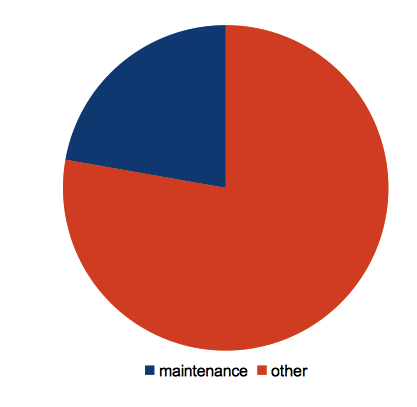
\includegraphics[width=0.5\textwidth]{termpaper/images/pie-chart-01}
\end{figure*}

\begin{figure*}[tbp!]
  \caption{Percentage of time spent on maintenance in Software Engineering major courses (approximate).}
  \centering
    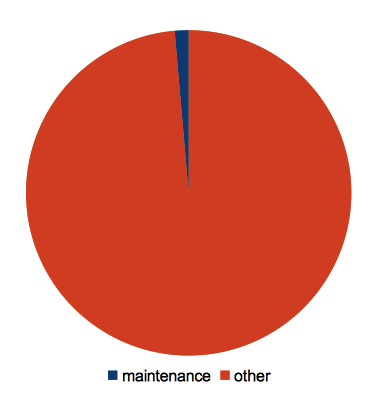
\includegraphics[width=0.5\textwidth]{termpaper/images/pie-chart-02}
\end{figure*}

\begin{figure*}[tbp!]
  \caption{Percentage of time spent on maintenance in Software Engineering all courses (approximate).}
  \centering
    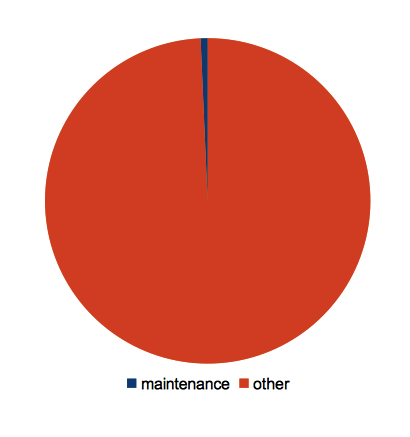
\includegraphics[width=0.5\textwidth]{termpaper/images/pie-chart-03}
\end{figure*}

As mentioned previously, professional studies have estimated 50-80 percent of a Software Engineer's working time is spent working on software maintenance. \cite{stark97} \cite{parekh}

\begin{figure*}[tbp!]
  \caption{Conservative estimate of working time spent in software maintenance as a Software Engineer.}
  \centering
    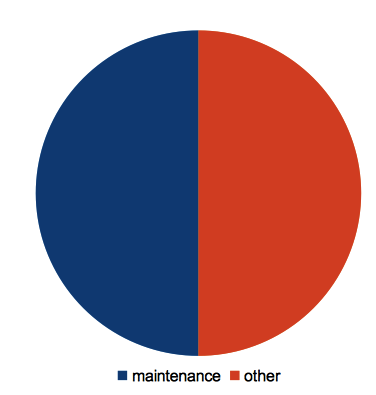
\includegraphics[width=0.5\textwidth]{termpaper/images/pie-chart-04}
\end{figure*}

Using the most conservative end of this estimation, we can say that the percentage of working time spent in software maintenance by professional Software Engineers is \emph{over 36 times more} than that spent in instruction in the Software Engineering program at Cal Poly.

Given these facts, it appears the department is not accurate in stating that Software Engineering students experience ``significant learning'' in software maintenance.

\subsubsection{Ethical Analysis}

If we can consider the Computer Science department to be equivalent to a student's manager or leader and the term of their enrollment to be employment, the department violates section 5.06 of the Software Engineering Code of Ethics by not accurately representing the amount of software maintenance done by students in the Software Engineering program.

A rule utilitarian will hold that Computer Science departments like Cal Poly's should hold to the SE Code when they can; regular breaking of the rules leads to societal distrust of the profession, which produces less happiness for both Software Engineers and those distrusting them.

In addition, section 1.6 of the SE code tells Software Engineers to

\begin{quote}
Be fair and avoid deception in all statements, particularly public ones, concerning software or related documents, methods and tools. \cite{secode}
\end{quote}

The courses required for a Software Engineering undergrad are part of a software engineering teaching method; thus, section 1.6 commands the Computer Science department to avoid deception when making statements about its Software Engineering program.

If, as previously determined, the program is not providing ``significant learning'' in software maintenance, as the department claims, the Computer Science department is making deceptive statements to current and prospective students about the Software Engineering program.

Section 1 of the Code regards ``the public interest'' and the subsections contained within are particulars about that subject. \cite{secode}  Utilitarianism is, in its essence, concerned with the public good. \cite{utilitarianism}  Rule utilitarianism in particular emphasizes conformance to rules unless given a strong reason to not.  Therefore, rule utilitarianism would find unethical the Computer Science department's lack of adherence to Section 1.6 and, following, Section 5.06.


%% Ensure Qualification
\subsection{Ensure Qualification}

Section 3.04 of the Software Engineering Code states that a professional Software Engineer must

\begin{quote}
Ensure that they are qualified for any project on which they work or propose to work by an appropriate combination of education and training, and experience. \cite{secode}
\end{quote}

This section is the first building block to analyzing the Computer Science department's behavior according to Section 5.11 of the Software Engineering Code.  To this end, it will show that Cal Poly's Software Engineering students are not encouraged or assisted in meeting this standard in regards to software maintenance.

We ask the reader to please remain patient as this multi-layered argument is established.

\subsubsection{Applicability of the Code}

The Computer Science Department claims that ``[t]he BS in Software Engineering prepares students to become software professionals''. \cite{catalogDept}  In addition, Cal Poly Software Engineering alumni frequently go on to pursue professional software development in industry. \cite{polyAlums}  Therefore, the Software Engineering Code applies to students in the Software Engineering program.

\subsubsection{Qualification}

A joint group from the Association for Computing Machinery (ACM) and Institute of Electrical and Electronics Engineers (IEEE) compiled a report (entitled ``Software Engineering 2004'') to ``provide guidance to academic institutions and accreditation agencies about what should constitute an undergraduate software engineering education''. \cite{se2004}  The report includes recommendations of minimum time to be spent covering certain topics; recognizing that lecture hours are a poor representation of absolute time, given the differences in instructional styles, the authors suggest that the hours should instead be viewed on a relative basis (that is, compared to each other to produce a percentage of time).

Out of the total 494 instructional hours, the report states that at least 10 should be spent on ``Software Evolution''.  The authors equate this to software maintenance:

\begin{quote}
Software ``maintenance'' primarily refers to continued development, or evolution, and not to conventional wear and tear. \cite{se2004}
\end{quote}

In addition, 13 hours are recommended for instruction in ``Software Process'':

\begin{quote}
Software process is concerned with knowledge about the description of commonly used software life-cycle process models and the contents of institutional process standards; definition, implementation, measurement, management, change and improvement of software processes; and \emph{use of a defined process to perform the technical and managerial activities needed for software development and maintenance} (emphasis added). \cite{se2004}
\end{quote}

And 16 hours are recommended for ``Software Quality'':

\begin{quote}
Software quality is a pervasive concept that affects, and is affected by all aspects of software development, support, revision, and \emph{maintenance}. It encompasses the quality of work products developed and/or modified [...] (emphasis added) \cite{se2004}
\end{quote}

While giving descriptions of potential course outlines, the authors of Software Engineering 2004 mention that they are basing their work upon a 40-hour course structure. \cite{se2004}  Cal Poly's Software Engineering degree requires roughly 24 courses under the ``Major Courses'' section \cite{catalogDegree}; 494 total hours divided by 24 courses gives us 20 hours per course.  To correctly compare Software Engineering 2004's hour recommendations with the hours Cal Poly students will experience, we must double SE2004's given hourly units.

As stated previously, we estimate that one-sixth of two standard four-unit courses in a Software Engineering undergraduate degree is spent discussing software maintenance.  Assuming again a 40-hour total course instructional time, less than 14 hours are spent discussing the subject.

When examining only the ``Software Evolution'' section of the report's recommendations, Cal Poly Software Engineering students should be receiving at least 20 hours of time being instructed in software maintenance.  In reality, this number should probably be much higher, since some of the 26 hours for ``Software Process'' and 32 hours for ``Software Quality'' would also count as instruction in this area.

Given the disparity between actual instructional hours and those recommended by Software Engineering 2004, we can say that students in Cal Poly's Software Engineering program are not qualified for software maintenance activities upon graduation.


%% Assist Colleagues in Professional Development
\subsection{Assist Colleagues in Professional Development}

Section 7 of the Software Engineering Code relates to a Software Engineer's behavior in relation to their colleagues:

\begin{quote}
%7.01. Encourage colleagues to adhere to this Code. \\
7.02. Assist colleagues in professional development.\cite{secode}
\end{quote}

\subsubsection{Applicability of the Code}

The preamble to the Code explicitly states that it applies to those engaged in the education of software engineers:

\begin{quote}
Software engineers are those who contribute by direct participation or by teaching, to the analysis, specification, design, development, certification, maintenance and testing of software systems. \cite{secode}
\end{quote}

Thus, the Code applies to professors in the Computer Science department at Cal Poly.

\subsubsection{Colleagues}

The Oxford Dictionary defines a colleague as

\begin{quote}
a person with whom one works in a profession or business. \cite{definitionColleague}
\end{quote}

As discussed in the previous section 4.2.1 (School vs. Employment), a working parallel regarding school as an employment can be set up for the purposes of this paper.  In this understanding, professors are the direct bosses over students.  Thus, we can say that students and teachers work with each other in a business.

Also, students are included by the Software Engineering Code as professional Software Engineers:

\begin{quote}
The Code contains eight Principles related to the behavior of and decisions made by professional software engineers, including practitioners, educators, managers, supervisors and policy makers, \emph{as well as trainees and students of the profession} (emphasis added). \cite{secode}
\end{quote}

Therefore, students and professors are colleagues through working in a common profession (software engineering).

\subsubsection{Assisting Colleagues}

The ACM and IEEE have collaboratively produced ``a consensually validated characterization of the bounds of the software engineering discipline'' in a document known as the Software Engineering Body of Knowledge (SWEBOK). \cite{swebok}  The SWEBOK consists of 10 knowledge areas, one of which is software maintenance. \cite{swebok}

As previously discussed in section 4.3 (Ensure Qualification), students in the Software Engineering program are receiving less education in software maintenance than recommended by the Software Engineering 2004 report; this puts them at a disadvantage when they try to fulfill the requirements of the SWEBOK in the years to come.

Therefore, to assist their students in professional development, professors at Cal Poly need to spend more class time covering software maintenance; currently, the professors are not following Software Engineering Code Section 7.02 fully.


%% Don't Ask for Code-Inconsistent Behavior
\subsection{Don't Ask for Code-Inconsistent Behavior}

Section 5.11 of the Software Engineering Code states that

\begin{quote}
[T]hose managing or leading software engineers shall [...] not ask a software engineer to do anything inconsistent with this Code. \cite{secode}
\end{quote}

\subsubsection{Applicability of the SE Code}

As previously discussed in section 4.1 (Applicability of the SE Code), the Code applies in general to the Computer Science department as an educator.

For this particular analysis, we have shown in section 4.4.1 (Applicability of the Code) that the professors in the Computer Science department are considered software engineers under the Code.  The department then, as their employer, qualifies for SE Code-applicability as one ``managing or leading software engineers''. \cite{secode}

\subsubsection{Asking for Code-Inconsistent Behavior}

As discussed in section 4.4 (Assist Colleagues in Professional Development), professors in Cal Poly's Computer Science department are not fully following Section 7.02 of the Code due to not spending enough course time teaching software maintenance to students.  By telling professors which courses to teach, the department is then asking them to continue engaging in this non-compliant behavior.

\subsubsection{Ethical Analysis}

Rule utilitarianism prefers adherence to rules considered to be generally causing the most good. \cite{ruleUtilitarianism}  The Software Engineering Code of Ethics was produced and approved by two professional societies, the IEEE and the ACM. \cite{secode}  If the Computer Science department causes less adherence to the Code through its course offerings, its actions would be considered unethical by a rule utilitarian for breaking a rule that has been agreed upon to help the Software Engineering profession.


%%%%%%%%%%%%%%%%
%%% Conclusion %%%
%%%%%%%%%%%%%%%%
\section{Conclusion}

Cal Poly's Computer Science department claims to prepare Software Engineering students to be professionals in the field of software engineering and to teach them in a number of subjects, including software maintenance. \cite{catalogDept}  There are a number of arguments as to why the department is currently doing a sufficient job - a maintenance-focused course is difficult to instruct, new courses incur both monetary and educational costs, and restructing an existing course to provide more of a focus on software maintenance would require less time spent on other subjects.

However, a number of professional software engineers have expressed the importance of software maintenance instruction.  In addition, best estimates show that the percentage of time spent in the field doing software maintenance as a professional software engineer vastly overshadows the percentage of time a Cal Poly Software Engineering student will spend learning how to do maintenance.

Given these two opposing sets of arguments, we ask the question ``Is the Computer Science department spending enough time teaching its Software Engineering students about software maintenance?''.

To answer this question, we applied sections 5.06, 1.6, 3.04, 7.02 and 5.11 of the Software Engineering Code of Ethics to information gathered from professional sources and the department itself.

Given the resulting analysis of the department's (lack of) conformance to the Code, we determined using the ethical system of utilitarianism that the department is acting unethically in regards to its current treatment of software maintenance.

%end the two column format
\end{multicols}
\newpage

%cite all the references from the bibtex you haven't explicitly cited
\nocite{*}

\bibliographystyle{termpaper/IEEEannot}

\bibliography{termpaper/texreport}

\end{document}
